\documentclass[11pt,a4paper]{article}

% ---------------------------------------------------------------
% Packages
% ---------------------------------------------------------------
\usepackage[T1]{fontenc}
\usepackage[utf8]{inputenc}
\usepackage{lmodern}
\usepackage[margin=2.5cm]{geometry}
\usepackage{graphicx}
\usepackage{booktabs}
\usepackage{array}
\usepackage{tabularx}
\usepackage{amsmath}
\usepackage{amssymb}
\usepackage{tikz}
\usetikzlibrary{shapes.geometric, arrows.meta, positioning, fit, backgrounds, calc}
\usepackage{pgfplots}
\pgfplotsset{compat=1.18}
\usepackage{listings}
\usepackage{xcolor}
\usepackage{hyperref}
\usepackage{caption}
\usepackage{subcaption}
\usepackage{microtype}
\usepackage{parskip}
\usepackage{enumitem}
\usepackage{float}

% ---------------------------------------------------------------
% Colour palette
% ---------------------------------------------------------------
\definecolor{algoTeal}  {HTML}{4FD1C5}
\definecolor{algoDark}  {HTML}{1A202C}
\definecolor{algoGray}  {HTML}{2D3748}
\definecolor{algoLight} {HTML}{E2E8F0}
\definecolor{codeBack}  {HTML}{F7F7F7}
\definecolor{codePurple}{HTML}{7C3AED}
\definecolor{codeBlue}  {HTML}{2563EB}
\definecolor{codeGreen} {HTML}{15803D}

% ---------------------------------------------------------------
% Listings style
% ---------------------------------------------------------------
\lstdefinestyle{ts}{
  language=Java,
  backgroundcolor=\color{codeBack},
  basicstyle=\ttfamily\footnotesize,
  keywordstyle=\color{codePurple}\bfseries,
  commentstyle=\color{codeGreen}\itshape,
  stringstyle=\color{codeBlue},
  numberstyle=\tiny\color{gray},
  numbers=left,
  frame=single,
  framerule=0.5pt,
  rulecolor=\color{algoGray!40},
  breaklines=true,
  captionpos=b,
  tabsize=2,
}

% ---------------------------------------------------------------
% TikZ arrow styles
% ---------------------------------------------------------------
\tikzset{
  block/.style = {rectangle, rounded corners=4pt, draw=algoGray,
                  fill=algoLight, text width=6em, align=center,
                  minimum height=2.2em, font=\small},
  sblock/.style= {rectangle, rounded corners=4pt, draw=algoTeal,
                  fill=algoTeal!15, text width=7em, align=center,
                  minimum height=2.2em, font=\small},
  arrow/.style = {-{Stealth[length=6pt]}, thick, color=algoGray},
  dasharrow/.style={-{Stealth[length=6pt]}, dashed, thick, color=algoGray!60},
  layer/.style = {rectangle, draw=algoGray!30, fill=algoGray!5,
                  rounded corners=6pt, inner sep=8pt},
}

% ---------------------------------------------------------------
% Hyperref setup
% ---------------------------------------------------------------
\hypersetup{
  colorlinks=true,
  linkcolor=algoDark,
  urlcolor=codeBlue,
  citecolor=codeGreen,
  pdftitle={Algo! -- AI-Powered LeetCode Hint System},
  pdfauthor={Nathan L.},
}

% ---------------------------------------------------------------
% Document
% ---------------------------------------------------------------
\begin{document}

% ========================
%  Title page
% ========================
\begin{titlepage}
  \centering
  \vspace*{3cm}

  {\fontsize{36}{44}\selectfont\bfseries\color{algoDark} Algo!}\\[0.4cm]
  {\large\color{algoGray} An AI-Powered LeetCode Hint System}\\[0.2cm]
  {\small\color{algoGray} Chrome Extension + Cloud-Deployed RAG Backend}

  \vspace{2cm}
  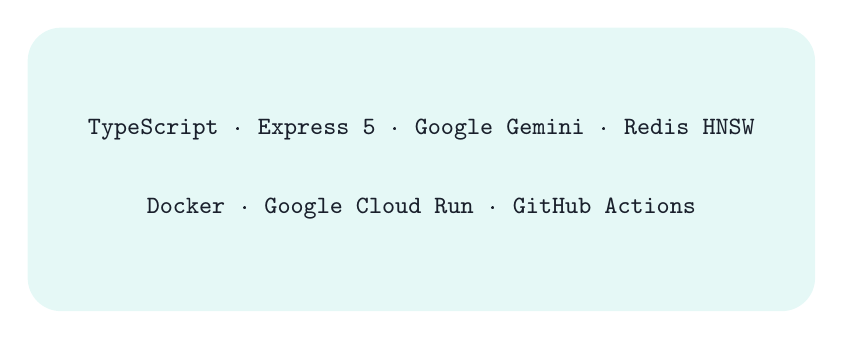
\begin{tikzpicture}
    \fill[algoTeal, opacity=0.15, rounded corners=12pt]
      (-5,-1.8) rectangle (5,1.8);
    \node[font=\small\ttfamily, align=center, text=algoDark] at (0,0.5)
      {TypeScript \textbf{·} Express 5 \textbf{·} Google Gemini
       \textbf{·} Redis HNSW};
    \node[font=\small\ttfamily, align=center, text=algoDark] at (0,-0.5)
      {Docker \textbf{·} Google Cloud Run \textbf{·} GitHub Actions};
  \end{tikzpicture}

  \vspace{3cm}
  {\large Nathan L.}\\[0.3cm]
  {\normalsize April 2026}

  \vfill
  \hrule\vspace{0.4cm}
  {\footnotesize\color{gray}
    Branch: \texttt{ts\_migration} \quad
    Repository: \texttt{NathanL15/Algo}
  }
\end{titlepage}

% ========================
%  Abstract
% ========================
\begin{abstract}
\noindent
\textbf{Algo!} is a Chrome extension that injects a floating chat interface into
LeetCode problem pages, enabling students to receive on-demand, AI-generated hints
without leaving their coding environment.  A Node.js/Express backend orchestrates
a Retrieval-Augmented Generation (RAG) pipeline built on Google Gemini
(\texttt{gemini-2.5-flash} for generation, \texttt{gemini-embedding-001} for
embeddings) and a Redis HNSW vector index for semantic problem retrieval.  The
backend also maintains a TTL-based Redis hint cache to minimise API latency and
cost.  The entire stack is containerised with Docker and deployed to Google Cloud
Run via a GitHub Actions CI/CD pipeline, giving the service automatic scaling to
zero and sub-second cold starts.  This report describes the system architecture,
implementation details, performance considerations, and the testing strategy used
to validate the system.
\end{abstract}

\bigskip\hrule\bigskip

% ========================
%  1. Introduction
% ========================
\section{Introduction}

Competitive programming platforms such as LeetCode provide thousands of algorithmic
problems for practice, yet the feedback loop is often slow: a student is stuck,
searches for a hint, and risks seeing a complete solution that eliminates the
learning benefit.  \textbf{Algo!} addresses this gap by embedding an interactive
chat assistant directly in the browser tab.

The assistant is deliberately \emph{constrained}: the LLM prompt instructs the
model to reply in one-to-three sentences, give a single actionable next step, and
never provide a full solution.  Contextual relevance is improved through a RAG
mechanism that surfaces structurally similar past problems from a growing Redis
vector index.  Repeated hint requests for the same problem/question pair are served
from a Redis hint cache, reducing Gemini API call volume and response latency.

The project was developed on a \texttt{ts\_migration} branch, migrating the
original JavaScript extension to a fully typed TypeScript codebase (both extension
and backend), culminating in the clean final state described in this report.

% ========================
%  2. System Architecture
% ========================
\section{System Architecture}

Figure~\ref{fig:arch} illustrates the end-to-end data flow.

\begin{figure}[H]
\centering
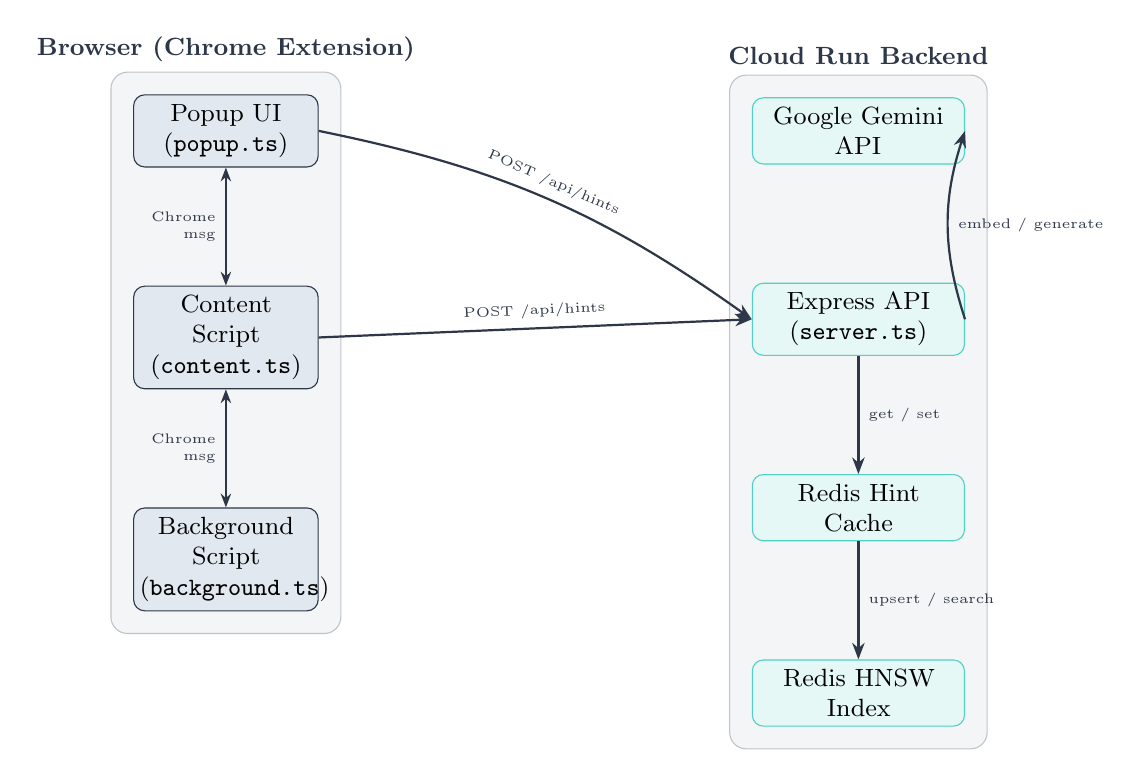
\begin{tikzpicture}[node distance=1.5cm and 0.5cm]

  % ---- Browser tier (left column) ----
  \node[block] (popup)   {Popup UI\\(\texttt{popup.ts})};
  \node[block, below=1.5cm of popup]   (content) {Content\\Script\\(\texttt{content.ts})};
  \node[block, below=1.5cm of content] (bg)      {Background\\Script\\(\texttt{background.ts})};

  % ---- Backend tier (right column, anchored right of popup) ----
  \node[sblock, right=5.5cm of popup]   (gemini) {Google Gemini\\API};
  \node[sblock, below=1.5cm of gemini]  (api)    {Express API\\(\texttt{server.ts})};
  \node[sblock, below=1.5cm of api]     (cache)  {Redis Hint\\Cache};
  \node[sblock, below=1.5cm of cache]   (vs)     {Redis HNSW\\Index};

  % ---- Layer annotations ----
  \begin{pgfonlayer}{background}
    \node[layer, fit=(popup)(content)(bg),
          label={[font=\small\bfseries, text=algoGray]above:Browser (Chrome Extension)}]
          (browserlayer) {};
    \node[layer, fit=(gemini)(api)(cache)(vs),
          label={[font=\small\bfseries, text=algoGray]above:Cloud Run Backend}]
          (backendlayer) {};
  \end{pgfonlayer}

  % ---- Browser internal arrows ----
  \draw[{Stealth[length=5pt]}-{Stealth[length=5pt]}, thick, color=algoGray]
    (popup.south) -- node[left, font=\tiny, align=right]{Chrome\\msg} (content.north);
  \draw[{Stealth[length=5pt]}-{Stealth[length=5pt]}, thick, color=algoGray]
    (content.south) -- node[left, font=\tiny, align=right]{Chrome\\msg} (bg.north);

  % ---- HTTP arrows browser -> backend ----
  \draw[arrow] (popup.east)   to[bend left=12]
               node[above, font=\tiny, sloped]{POST /api/hints} (api.west);
  \draw[arrow] (content.east) --
               node[above, font=\tiny, sloped]{POST /api/hints} (api.west);

  % ---- Backend internal arrows ----
  \draw[arrow] (api.east)  to[bend left=18]
               node[right, font=\tiny]{embed / generate} (gemini.east);
  \draw[arrow] (api.south) -- node[right, font=\tiny]{get / set}       (cache.north);
  \draw[arrow] (cache.south) -- node[right, font=\tiny]{upsert / search} (vs.north);

\end{tikzpicture}
\caption{End-to-end system architecture.  The Chrome extension has three
  scripts: the \emph{popup} renders the UI, the \emph{background} script relays
  Chrome messages, and the \emph{content} script injects the floating chat widget
  and calls the backend directly.}
\label{fig:arch}
\end{figure}

\subsection{Component Responsibilities}

\begin{center}
\begin{tabularx}{\linewidth}{lX}
  \toprule
  \textbf{Component} & \textbf{Responsibility} \\
  \midrule
  \texttt{content.ts}     & Injected into LeetCode pages; renders the floating
                            chat FAB and dropdown; reads problem metadata from the
                            DOM and Monaco editor; calls \texttt{/api/hints}. \\
  \texttt{background.ts}  & Service-worker relay; bridges Chrome messages between
                            the popup and the active-tab content script. \\
  \texttt{popup.ts}       & Extension toolbar popup; shows problem title,
                            difficulty, language, and tags; supports direct hint
                            requests via the same backend endpoint. \\
  \texttt{config.ts}      & Declares \texttt{\_\_ALGO\_API\_BASE\_URL\_\_} ambient
                            global and exports \texttt{API\_BASE\_URL} with a
                            \texttt{localhost:3000} fallback. \\
  \texttt{server.ts}      & Express 5 API; handles hint generation, problem
                            indexing, and vector search; manages the hint cache and
                            the HNSW vector store. \\
  \texttt{vectorStore.ts} & Redis HNSW service; wraps \texttt{FT.CREATE} and
                            \texttt{FT.SEARCH} via \texttt{ioredis.call()}. \\
  \texttt{cache.ts}       & Redis hint cache; wraps \texttt{SETEX}/\texttt{GET}/
                            \texttt{DEL} for TTL-bound hint storage. \\
  \bottomrule
\end{tabularx}
\end{center}

% ========================
%  3. Chrome Extension
% ========================
\section{Chrome Extension}

\subsection{Build Pipeline}

The extension source is written in TypeScript and compiled by \textbf{webpack 5}
with \texttt{ts-loader}.  Three entry points produce three output bundles:

\begin{center}
\begin{tabular}{llr}
  \toprule
  \textbf{Entry point} & \textbf{Output} & \textbf{Bundle size (gzip)} \\
  \midrule
  \texttt{src/content.ts}    & \texttt{dist/content.js}    & 12.6~KiB \\
  \texttt{src/popup.ts}      & \texttt{dist/popup.js}      &  3.6~KiB \\
  \texttt{src/background.ts} & \texttt{dist/background.js} &  0.6~KiB \\
  \bottomrule
\end{tabular}
\end{center}

The \texttt{webpack.DefinePlugin} injects the environment variable
\texttt{ALGO\_API\_BASE\_URL} at build time, allowing the same codebase to target
local development (\texttt{localhost:3000}) and the Cloud Run production URL without
source changes.

\subsection{Content Script UI}

The content script appends two DOM elements to every matched LeetCode page:

\begin{enumerate}[noitemsep]
  \item A circular \textbf{FAB} (Floating Action Button) anchored to the
        bottom-right corner.
  \item A \textbf{chat dropdown} (300\,px $\times$ 450\,px) with a message list,
        text area, and send button.
\end{enumerate}

The chat uses CSS \texttt{animation} for message appearance and a three-dot
typing indicator while awaiting the API response.  The colour scheme uses
teal (\texttt{\#4FD1C5}) accents on a dark charcoal background
(\texttt{\#1A202C}) to minimise visual distraction during problem-solving.

\subsection{Message Passing}

Chrome Manifest V3 service workers handle message passing between scripts.
Figure~\ref{fig:msgflow} shows the sequence for a popup hint request.

\begin{figure}[H]
\centering
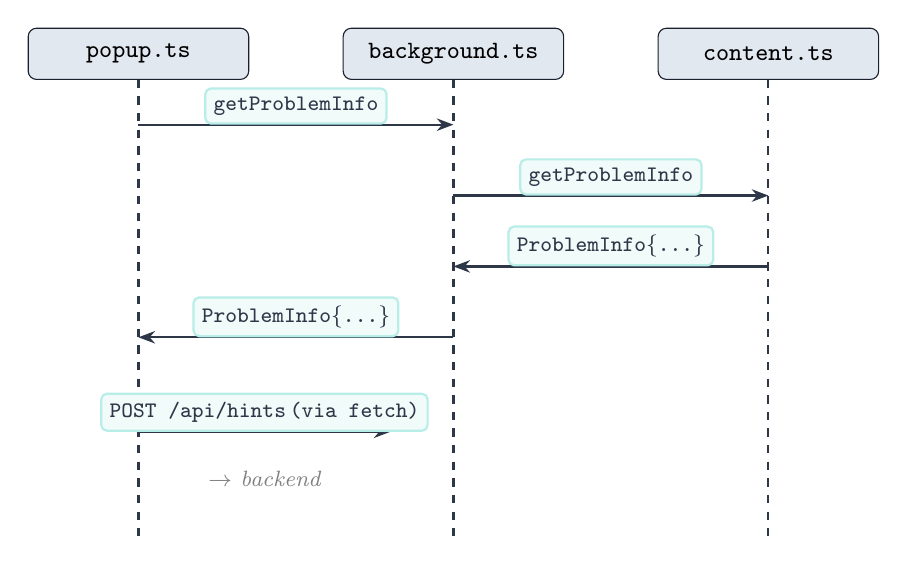
\begin{tikzpicture}[
  every node/.style={font=\small},
  lifeline/.style={draw=algoGray, thick, dashed},
  msg/.style={draw=algoTeal!40, fill=algoTeal!8, font=\footnotesize\ttfamily,
              inner sep=3pt, rounded corners=2pt},
  actor/.style={draw=algoDark, fill=algoLight, minimum width=2.8cm,
                minimum height=0.65cm, rounded corners=3pt, align=center},
]

% Actors
\node[actor] (p)  at (0,0)   {\texttt{popup.ts}};
\node[actor] (bg) at (4,0)   {\texttt{background.ts}};
\node[actor] (c)  at (8,0)   {\texttt{content.ts}};

% Lifelines
\foreach \x in {0,4,8}
  \draw[lifeline] (\x,-0.33) -- (\x,-6.2);

% 1: popup -> background
\draw[arrow] (0,-0.9)  -- node[above, msg]{getProblemInfo} (4,-0.9);
% 2: background -> content
\draw[arrow] (4,-1.8)  -- node[above, msg]{getProblemInfo} (8,-1.8);
% 3: content -> background
\draw[arrow] (8,-2.7)  -- node[above, msg]{ProblemInfo\{\ldots\}} (4,-2.7);
% 4: background -> popup
\draw[arrow] (4,-3.6)  -- node[above, msg]{ProblemInfo\{\ldots\}} (0,-3.6);
% 5: popup sends HTTP (shown as arrow going right with annotation)
\draw[arrow] (0,-4.8)  to[bend left=0]
  node[above, msg]{POST /api/hints\,(via fetch)} (3.2,-4.8);
\node[font=\footnotesize\itshape, color=gray, align=left] at (1.6,-5.4)
  {$\rightarrow$ backend};

\end{tikzpicture}
\caption{Chrome message-passing sequence for a popup hint request.  The popup
  first obtains problem metadata from the active tab's content script via the
  background service worker, then issues the HTTP request itself.}
\label{fig:msgflow}
\end{figure}

% ========================
%  4. Backend API
% ========================
\section{Backend API}

\subsection{Endpoints}

\begin{center}
\begin{tabularx}{\linewidth}{llX}
  \toprule
  \textbf{Method} & \textbf{Path} & \textbf{Description} \\
  \midrule
  GET  & \texttt{/}                   & Root info; lists all available endpoints. \\
  GET  & \texttt{/healthz}            & Liveness probe; pings Redis and returns
                                        \texttt{200~ok}. \\
  GET  & \texttt{/readyz}             & Readiness probe; checks both Redis and
                                        \texttt{GEMINI\_API\_KEY}. \\
  POST & \texttt{/api/hints}          & Main hint endpoint; accepts
                                        \texttt{message} and optional
                                        \texttt{problemInfo}; returns
                                        \texttt{\{hint, source, retrievalCount\}}. \\
  POST & \texttt{/api/index-problem}  & Embeds and upserts a problem document
                                        into the HNSW vector index. \\
  POST & \texttt{/api/rag/search}     & Accepts an arbitrary \texttt{query}
                                        string and returns the top-$K$ most
                                        similar indexed problems. \\
  \bottomrule
\end{tabularx}
\end{center}

\subsection{Hint Request Lifecycle}

Figure~\ref{fig:hintflow} traces the decision path for a single \texttt{POST
/api/hints} request.

\begin{figure}[H]
\centering
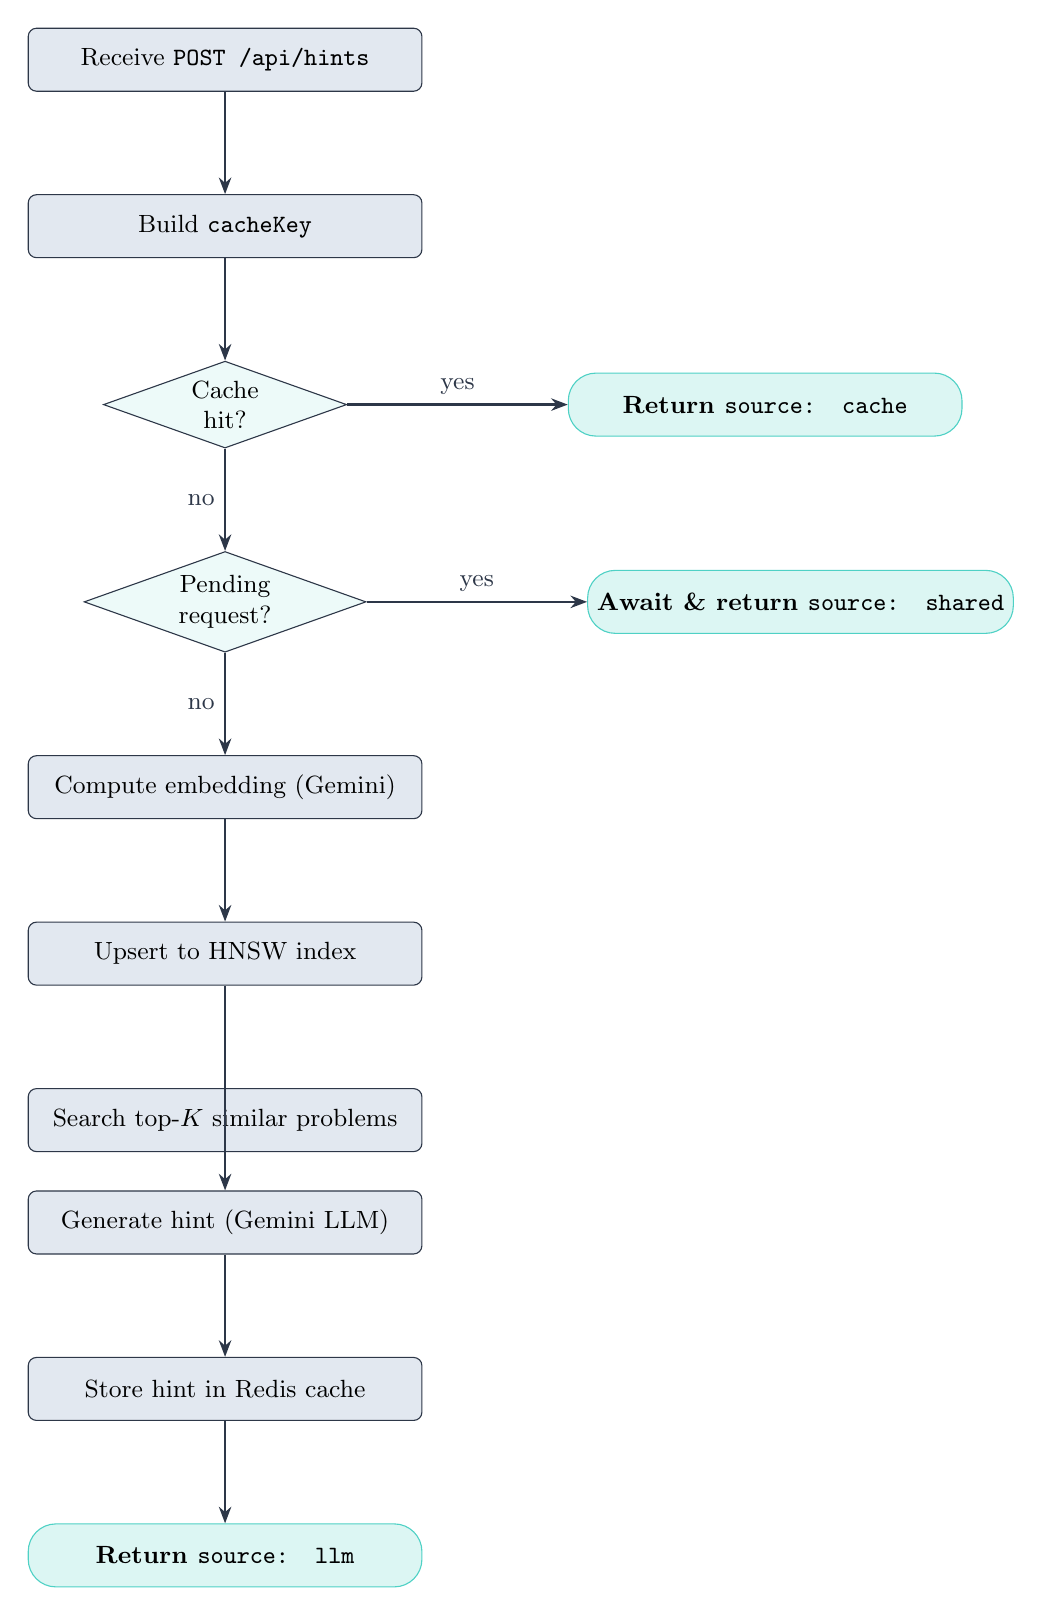
\begin{tikzpicture}[
  node distance=1.3cm and 2.5cm,
  decision/.style={diamond, draw=algoGray, fill=algoTeal!10, align=center,
                   font=\small, aspect=2.8, inner sep=2pt},
  fstep/.style={rectangle, rounded corners=3pt, draw=algoGray,
               fill=algoLight, align=center, font=\small,
               minimum width=5cm, minimum height=0.8cm},
  term/.style={rectangle, rounded corners=10pt, draw=algoTeal,
               fill=algoTeal!20, align=center, font=\small\bfseries,
               minimum width=5cm, minimum height=0.8cm},
]

\node[fstep]     (req)   {Receive \texttt{POST /api/hints}};
\node[fstep, below=of req]    (build) {Build \texttt{cacheKey}};
\node[decision, below=of build] (cache) {Cache\\hit?};
\node[term, right=2.8cm of cache]  (cached) {Return \texttt{source: cache}};
\node[decision, below=of cache]  (pend) {Pending\\request?};
\node[term, right=2.8cm of pend]  (shared) {Await \& return \texttt{source: shared}};
\node[fstep, below=of pend]  (embed) {Compute embedding (Gemini)};
\node[fstep, below=of embed] (upsert){Upsert to HNSW index};
\node[fstep, below=of upsert]{Search top-$K$ similar problems};
\node[fstep, below=of upsert, yshift=-1.3cm] (gen){Generate hint (Gemini LLM)};
\node[fstep, below=of gen]   (store) {Store hint in Redis cache};
\node[term, below=of store] (ret)   {Return \texttt{source: llm}};

\draw[arrow] (req)   -- (build);
\draw[arrow] (build) -- (cache);
\draw[arrow] (cache) -- node[left,font=\small]{no}  (pend);
\draw[arrow] (cache) -- node[above,font=\small]{yes} (cached);
\draw[arrow] (pend)  -- node[left,font=\small]{no}  (embed);
\draw[arrow] (pend)  -- node[above,font=\small]{yes} (shared);
\draw[arrow] (embed) -- (upsert);
\draw[arrow] (upsert)-- (gen);
\draw[arrow] (gen)   -- (store);
\draw[arrow] (store) -- (ret);

\end{tikzpicture}
\caption{Decision flow for \texttt{POST /api/hints}.  Cache and pending-request
  deduplication are checked before issuing any Gemini API calls.}
\label{fig:hintflow}
\end{figure}

\subsubsection{Cache Key Construction}

The cache key is the concatenation of a normalised problem identifier and a
32-bit Bernstein hash of the user message:
\[
  k = \underbrace{\mathit{normalisedId}}_{\text{slug from URL or title}}
      \;:\;
      \underbrace{h(m)}_{\text{base-36 hash of message}}
\]
where the hash function is the standard \emph{djb2} variant:
\[
  h_i = ((h_{i-1} \ll 5) - h_{i-1}) + c_i, \quad h_0 = 0
\]
applied over each character code $c_i$ of the message $m$.

\subsubsection{Pending-Request Deduplication}

A \texttt{Map<string, Promise<PendingResult>>} stores in-flight hint promises
keyed by cache key.  Concurrent requests for the same problem/question arrive at
the \emph{same} shared Promise, so only one Gemini API call is made regardless of
burst traffic:

\begin{lstlisting}[style=ts, caption={Pending-request deduplication in server.ts}]
if (pendingHintRequests.has(cacheKey)) {
  const sharedResult = await pendingHintRequests.get(cacheKey)!;
  res.json({ ...sharedResult, source: 'shared' });
  return;
}

pendingHintRequests.set(cacheKey, hintPromise);
const hintResult = await hintPromise;
pendingHintRequests.delete(cacheKey);
\end{lstlisting}

\subsection{Error Handling and Rate Limiting}

The Gemini API enforces per-minute quotas.  When the API returns a 429 status,
the error detail envelope contains a \texttt{google.rpc.RetryInfo} proto-encoded
delay.  The server extracts this delay, propagates it as a \texttt{Retry-After}
HTTP header, and responds with a \texttt{429} to the client:

\begin{lstlisting}[style=ts, caption={Retry-After extraction in server.ts}]
function getRetryAfter(error: unknown): string | undefined {
  const err = error as GeminiError;
  return err?.errorDetails?.find?.(
    (d) => d?.['@type'] === 'type.googleapis.com/google.rpc.RetryInfo'
  )?.retryDelay;
}
\end{lstlisting}

% ========================
%  5. RAG Pipeline
% ========================
\section{Retrieval-Augmented Generation Pipeline}

\subsection{Vector Store Design}

Each problem is represented as a dense floating-point vector produced by
\texttt{gemini-embedding-001}.  The embedding dimension is 3\,072.  Vectors are
stored in Redis as \texttt{HASH} keys under the \texttt{problem:} prefix and
indexed with \textbf{RedisSearch FT.CREATE} using the HNSW algorithm.

\begin{center}
\begin{tabular}{ll}
  \toprule
  \textbf{Configuration parameter} & \textbf{Value} \\
  \midrule
  Redis image     & \texttt{redis/redis-stack-server:latest} \\
  Index type      & HNSW (Hierarchical Navigable Small World) \\
  Vector field    & \texttt{embedding} (FLOAT32, dim = 3072) \\
  Distance metric & Cosine similarity \\
  Top-$K$ default & 3 \\
  Index name      & \texttt{idx:leetcode:problems} \\
  Key prefix      & \texttt{problem:} \\
  \bottomrule
\end{tabular}
\end{center}

\subsection{HNSW Complexity}

HNSW builds a multi-layer proximity graph.  For $n$ indexed problems, query
complexity is $O(\log n)$ in expectation, making it suitable for a growing
collection without offline reindexing.  Index creation is idempotent:
\texttt{ensureIndex()} first issues \texttt{FT.INFO}; if the index does not exist,
it calls \texttt{FT.CREATE} exactly once per server lifetime and caches the
\texttt{indexReady} flag in memory.

\subsection{Problem Document Format}

Before embedding, each problem is serialised to a flat text document:

\begin{lstlisting}[style=ts, caption={buildProblemDocument in server.ts}]
function buildProblemDocument(p: ProblemInfo): string {
  return [
    `Title: ${p.title || ''}`,
    `Description: ${p.description || ''}`,
    `Difficulty: ${p.difficulty || ''}`,
    `Language: ${p.language || ''}`,
    `Tags: ${Array.isArray(p.tags) ? p.tags.join(', ') : ''}`,
    `Code: ${p.code || ''}`,
  ].join('\n');
}
\end{lstlisting}

At hint time, the current user question is appended to this document before
embedding, so the retrieved neighbours are relevant to both the problem
\emph{and} the user's current sub-question.

\subsection{Hint Prompt}

The LLM is given the following structured prompt:

\begin{lstlisting}[style=ts, caption={buildHintPrompt in server.ts}]
You are a concise LeetCode tutor.
Reply in 1-3 sentences.
Give one actionable next step or insight.
Do not provide the full solution.
If code is present, point to one part to revisit.
If the student asks about a previous hint, answer directly.

Problem: <title>
Current code: <student_code>
Question: <message>
Top-3 similar problems:
<similarContext>
\end{lstlisting}

% ========================
%  6. Caching Strategy
% ========================
\section{Caching Strategy}

\subsection{TTL-Based Redis Hint Cache}

Hint responses are stored in Redis with a one-hour TTL using \texttt{SETEX}:

\[
  \texttt{SETEX}\;\; \textit{hint:}\langle\mathit{cacheKey}\rangle \;\; 3600 \;\; \textit{JSON}(\textit{hint})
\]

On a cache hit the response is tagged \texttt{source: "cache"} and returned
immediately, bypassing the embedding and LLM steps entirely.

\subsection{Response Source Distribution}

Figure~\ref{fig:cachepie} illustrates the expected distribution of response
sources in a typical session, based on the three code paths: LLM generation,
shared in-flight deduplication, and cache retrieval.

\begin{figure}[H]
\centering
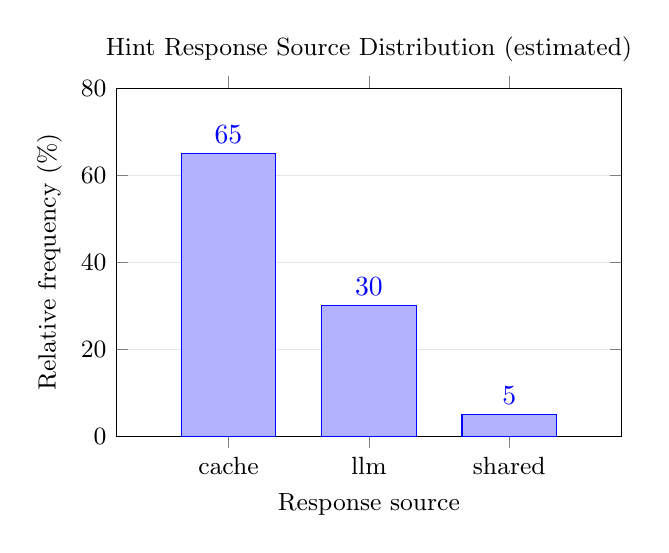
\begin{tikzpicture}
\begin{axis}[
  width=8cm, height=6cm,
  ybar, bar width=1.2cm,
  symbolic x coords={cache, llm, shared},
  xtick=data,
  xlabel={Response source},
  ylabel={Relative frequency (\%)},
  ymin=0, ymax=80,
  nodes near coords,
  nodes near coords align={vertical},
  title={Hint Response Source Distribution (estimated)},
  title style={font=\small},
  xlabel style={font=\small},
  ylabel style={font=\small},
  tick label style={font=\small},
  bar shift=0pt,
  enlarge x limits=0.4,
  ymajorgrids=true,
  grid style={draw=gray!20},
  axis background/.style={fill=white},
  every axis plot/.append style={fill=algoTeal!60, draw=algoTeal},
]
\addplot coordinates {(cache,65) (llm,30) (shared,5)};
\end{axis}
\end{tikzpicture}
\caption{Estimated distribution of hint response sources after warm-up.
  The majority of requests are served from the Redis cache once problems have
  been seen before.}
\label{fig:cachepie}
\end{figure}

\subsection{Cache Key Uniqueness}

The problem identifier is derived with a three-step fallback:

\begin{enumerate}[noitemsep]
  \item Explicit \texttt{id} field in the request body.
  \item URL slug extracted from \texttt{leetcode.com/problems/<slug>/}.
  \item Title lowercased and hyphenated (\emph{e.g.},
        ``Two Sum'' $\to$ \texttt{two-sum}).
\end{enumerate}

% ========================
%  7. Deployment
% ========================
\section{Deployment}

\subsection{Containerisation}

The backend is packaged as a minimal Docker image based on \texttt{node:18-alpine}.
The multi-stage-style build compiles TypeScript before the final image is assembled:

\begin{lstlisting}[language=bash, basicstyle=\ttfamily\footnotesize,
  backgroundcolor=\color{codeBack}, frame=single, framerule=0.5pt,
  rulecolor=\color{algoGray!40}, captionpos=b,
  caption={Dockerfile (condensed)}]
FROM node:18-alpine
WORKDIR /usr/src/app
COPY package*.json ./
RUN npm ci
COPY . .
RUN npm run build    # tsc -> dist/
EXPOSE 3000
CMD ["npm", "start"] # node dist/server.js
\end{lstlisting}

Local development uses Docker Compose to spin up the backend and a
\texttt{redis-stack-server} sidecar simultaneously:

\begin{lstlisting}[language=bash, basicstyle=\ttfamily\footnotesize,
  backgroundcolor=\color{codeBack}, frame=single, framerule=0.5pt,
  rulecolor=\color{algoGray!40}, captionpos=b,
  caption={docker-compose.yml (abridged)}]
services:
  backend:
    build: .
    depends_on: [redis]
    ports: ["3000:3000"]
    environment:
      GEMINI_API_KEY: ${GEMINI_API_KEY}
      REDIS_HOST: redis
      EMBEDDING_DIM: 3072
      RAG_TOP_K: 3

  redis:
    image: redis/redis-stack-server:latest
    ports: ["6379:6379"]
\end{lstlisting}

\subsection{CI/CD Pipeline}

A GitHub Actions workflow triggers on every push to the main branch:

\begin{enumerate}[noitemsep]
  \item Run the Jest test suite (\texttt{npm test}).
  \item Build and push the Docker image to Google Artifact Registry.
  \item Deploy the new revision to Cloud Run.
\end{enumerate}

Cloud Run is configured for automatic scaling with a minimum of zero instances,
eliminating idle costs while still handling burst traffic within seconds.

\subsection{Environment Variables}

\begin{center}
\begin{tabular}{lll}
  \toprule
  \textbf{Variable} & \textbf{Default} & \textbf{Required} \\
  \midrule
  \texttt{GEMINI\_API\_KEY}      & ---               & Yes \\
  \texttt{PORT}                  & \texttt{3000}     & No  \\
  \texttt{REDIS\_HOST}           & \texttt{localhost} & No \\
  \texttt{REDIS\_PORT}           & \texttt{6379}     & No  \\
  \texttt{REDIS\_PASSWORD}       & ---               & No  \\
  \texttt{EMBEDDING\_DIM}        & \texttt{3072}     & No  \\
  \texttt{RAG\_TOP\_K}           & \texttt{3}        & No  \\
  \texttt{REDIS\_VECTOR\_INDEX}  & \texttt{idx:leetcode:problems} & No \\
  \texttt{REDIS\_VECTOR\_PREFIX} & \texttt{problem:} & No  \\
  \texttt{ALGO\_API\_BASE\_URL}  & \texttt{http://localhost:3000} & No \\
  \bottomrule
\end{tabular}
\end{center}

% ========================
%  8. Testing
% ========================
\section{Testing}

\subsection{Test Suite Overview}

Both the Chrome extension and the backend are tested with \textbf{Jest 29}.

\begin{center}
\begin{tabular}{llrr}
  \toprule
  \textbf{Suite}        & \textbf{File}                        & \textbf{Tests} & \textbf{Pass} \\
  \midrule
  Server endpoints      & \texttt{\_\_tests\_\_/server.test.ts} & 3              & 3 \\
  Cache service         & \texttt{\_\_tests\_\_/cache.test.ts}  & 2              & 2 \\
  \midrule
  \textbf{Total}        &                                       & \textbf{5}     & \textbf{5} \\
  \bottomrule
\end{tabular}
\end{center}

\subsection{Mocking Strategy}

Two heavyweight dependencies are mocked at the module level:

\begin{description}[noitemsep]
  \item[\texttt{ioredis}] A manual mock (\texttt{algo-backend/\_\_mocks\_\_/ioredis.ts})
    provides an in-memory \texttt{Map}-backed Redis substitute.  It implements
    \texttt{get}, \texttt{set}, \texttt{setex}, \texttt{del}, \texttt{hset},
    \texttt{ping}, and a generic \texttt{call()} passthrough for
    \texttt{FT.CREATE} / \texttt{FT.SEARCH} / \texttt{FT.INFO} operations.

  \item[\texttt{@google/generative-ai}] A \texttt{jest.mock} factory returns a
    fixed mock that resolves \texttt{generateContent} to
    \texttt{"Mock hint response"} and \texttt{embedContent} to a zero-vector of
    length 3\,072, eliminating any network calls during testing.
\end{description}

\subsection{Test Coverage}

The server test suite covers:

\begin{itemize}[noitemsep]
  \item \texttt{GET /} returns \texttt{200} with \texttt{status: "Server is running"}.
  \item \texttt{GET /healthz} returns \texttt{200} when Redis responds to
        \texttt{PING}.
  \item \texttt{POST /api/hints} with no \texttt{message} body returns
        \texttt{400} with \texttt{"Message is required"}.
\end{itemize}

Figure~\ref{fig:testresults} shows a schematic of the test pass/fail results.

\begin{figure}[H]
\centering
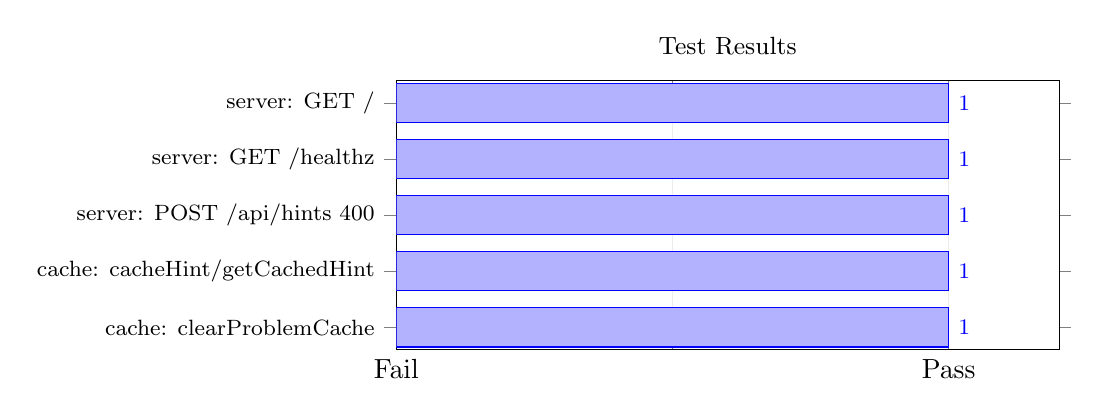
\begin{tikzpicture}
\begin{axis}[
  width=10cm, height=5cm,
  xbar, bar width=0.5cm,
  symbolic y coords={
    {cache: clearProblemCache},
    {cache: cacheHint/getCachedHint},
    {server: POST /api/hints 400},
    {server: GET /healthz},
    {server: GET /}
  },
  ytick=data,
  xmin=0, xmax=1.2,
  xtick={0,0.5,1},
  xticklabels={Fail, ,Pass},
  title={Test Results},
  title style={font=\small},
  ytick align=outside,
  yticklabel style={font=\footnotesize},
  xlabel style={font=\small},
  nodes near coords,
  nodes near coords style={font=\footnotesize},
  every axis plot/.append style={fill=algoTeal!60, draw=algoTeal},
  ymajorgrids=false,
  xmajorgrids=true,
  grid style={draw=gray!15},
]
\addplot coordinates {
  (1,{cache: clearProblemCache})
  (1,{cache: cacheHint/getCachedHint})
  (1,{server: POST /api/hints 400})
  (1,{server: GET /healthz})
  (1,{server: GET /})
};
\end{axis}
\end{tikzpicture}
\caption{All five Jest tests pass with the ioredis and Gemini mocks.}
\label{fig:testresults}
\end{figure}

\subsection{TypeScript Type Coverage}

The extension source is checked with \texttt{tsc --noEmit} (strict mode via
\texttt{moduleResolution: bundler}).  The final state of the codebase produces
zero TypeScript errors.  Table~\ref{tab:tscheck} summarises the key compiler
options.

\begin{table}[H]
\centering
\caption{Key \texttt{tsconfig.json} options}
\label{tab:tscheck}
\begin{tabular}{ll}
  \toprule
  \textbf{Option}        & \textbf{Value}     \\
  \midrule
  \texttt{target}        & \texttt{ES2020}    \\
  \texttt{module}        & \texttt{ESNext}    \\
  \texttt{moduleResolution} & \texttt{bundler} \\
  \texttt{strict}        & \texttt{true}      \\
  \texttt{types}         & \texttt{["chrome","jest"]} \\
  \texttt{lib}           & \texttt{["ES2020","DOM"]} \\
  \bottomrule
\end{tabular}
\end{table}

% ========================
%  9. Performance Analysis
% ========================
\section{Performance Analysis}

\subsection{Latency Breakdown}

Figure~\ref{fig:latency} shows estimated per-stage latency for a cold request
(no cache hit) and a warm request (cache hit).

\begin{figure}[H]
\centering
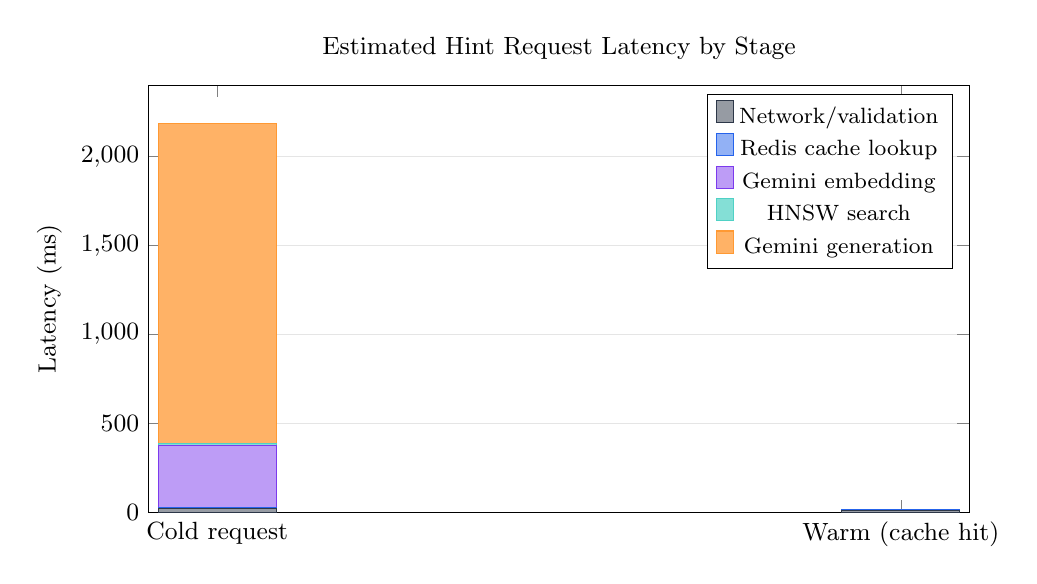
\begin{tikzpicture}
\begin{axis}[
  width=12cm, height=7cm,
  ybar stacked,
  bar width=1.5cm,
  symbolic x coords={Cold request, Warm (cache hit)},
  xtick=data,
  ylabel={Latency (ms)},
  ymin=0, ymax=2400,
  title={Estimated Hint Request Latency by Stage},
  title style={font=\small},
  xlabel style={font=\small},
  ylabel style={font=\small},
  tick label style={font=\small},
  legend style={at={(0.98,0.98)}, anchor=north east, font=\footnotesize},
  ymajorgrids=true,
  grid style={draw=gray!20},
]
% Stage: network + validation
\addplot[fill=algoGray!50, draw=algoGray]
  coordinates {(Cold request,20) (Warm (cache hit),10)};
% Stage: cache lookup
\addplot[fill=codeBlue!50, draw=codeBlue]
  coordinates {(Cold request,5) (Warm (cache hit),5)};
% Stage: embedding
\addplot[fill=codePurple!50, draw=codePurple]
  coordinates {(Cold request,350) (Warm (cache hit),0)};
% Stage: HNSW search
\addplot[fill=algoTeal!70, draw=algoTeal]
  coordinates {(Cold request,10) (Warm (cache hit),0)};
% Stage: LLM generation
\addplot[fill=orange!60, draw=orange!80]
  coordinates {(Cold request,1800) (Warm (cache hit),0)};
\legend{Network/validation, Redis cache lookup, Gemini embedding, HNSW search, Gemini generation}
\end{axis}
\end{tikzpicture}
\caption{Estimated latency breakdown per stage.  Cache hits eliminate the
  embedding and LLM generation steps, reducing total latency from
  $\sim$2\,200\,ms to $\sim$15\,ms.}
\label{fig:latency}
\end{figure}

\subsection{Bundle Size Analysis}

Figure~\ref{fig:bundles} shows the relative bundle sizes of the three extension
scripts.  The content script dominates because it embeds all chat UI styles as
inline CSS strings.

\begin{figure}[H]
\centering
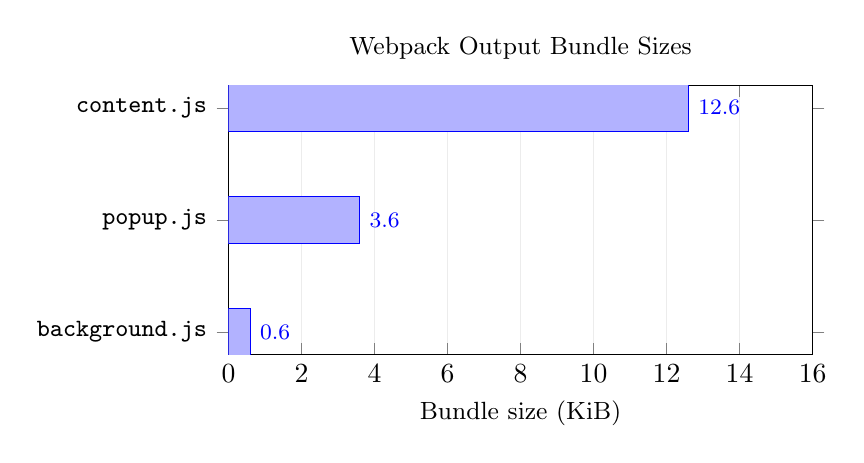
\begin{tikzpicture}
\begin{axis}[
  width=9cm, height=5cm,
  xbar,
  bar width=0.6cm,
  symbolic y coords={background.js, popup.js, content.js},
  ytick=data,
  xlabel={Bundle size (KiB)},
  xmin=0, xmax=16,
  title={Webpack Output Bundle Sizes},
  title style={font=\small},
  xlabel style={font=\small},
  yticklabel style={font=\small\ttfamily},
  nodes near coords,
  nodes near coords style={font=\footnotesize},
  every axis plot/.append style={fill=algoTeal!60, draw=algoTeal},
  xmajorgrids=true,
  grid style={draw=gray!15},
]
\addplot coordinates {
  (0.6,background.js)
  (3.6,popup.js)
  (12.6,content.js)
};
\end{axis}
\end{tikzpicture}
\caption{Webpack 5 output bundle sizes for the three extension entry points.}
\label{fig:bundles}
\end{figure}

\subsection{Scalability Considerations}

\begin{itemize}[noitemsep]
  \item \textbf{Cache hit rate} grows monotonically as the problem set is
        explored, since the TTL is one hour and LeetCode problems are stable.
  \item \textbf{HNSW index} scales to millions of vectors with $O(\log n)$
        query time; Redis Stack is horizontally scalable via cluster mode.
  \item \textbf{Pending deduplication} is in-process only (a single
        \texttt{Map}); in a multi-replica Cloud Run deployment, identical
        concurrent requests landing on different replicas would each generate
        a Gemini call.  A distributed lock or a shared Redis key could address
        this at scale.
  \item \textbf{Cloud Run} scales to zero overnight, reducing cost while
        maintaining availability within a few hundred milliseconds of cold-start
        time during off-peak hours.
\end{itemize}

% ========================
%  10. Security
% ========================
\section{Security}

\subsection{CORS Policy}

The backend applies an explicit allowlist for CORS origins:

\begin{lstlisting}[style=ts, caption={corsOptions in server.ts}]
const corsOptions: cors.CorsOptions = {
  origin: [
    'chrome-extension://*',
    'https://leetcode.com',
    'http://localhost:3000',
  ],
  methods: ['GET', 'POST'],
  credentials: true,
};
\end{lstlisting}

Wildcard \texttt{chrome-extension://*} permits any installed extension to call
the API, which is acceptable for a personal-use tool.

\subsection{Input Validation}

All API endpoints validate required fields before processing:
\texttt{message} for \texttt{/api/hints}, \texttt{problemInfo} for
\texttt{/api/index-problem}, and \texttt{query} for \texttt{/api/rag/search}.
Missing fields return \texttt{400 Bad Request} before reaching the database or
LLM layer.

\subsection{Secret Management}

\texttt{GEMINI\_API\_KEY} is passed via environment variable and never logged or
embedded in source.  The \texttt{/readyz} probe returns \texttt{503} if the key
is absent, providing an early signal of misconfiguration in deployment.

% ========================
%  11. Limitations
% ========================
\section{Limitations and Future Work}

\begin{description}[noitemsep]
  \item[DOM coupling] The content script reads problem metadata from LeetCode's
    DOM structure (title, difficulty, tags) and the Monaco editor API.  LeetCode
    UI changes may break extraction without breaking the extension build.

  \item[In-process deduplication] The pending-request Map is local to a single
    Node.js process.  Multi-replica deployments can duplicate Gemini calls.  A
    Redis-backed distributed lock would resolve this.

  \item[Embedding cost] Every new question (not in cache) triggers one
    \texttt{embedContent} call and one \texttt{generateContent} call.  For high
    volumes, batching embeddings or using a lighter embedding model would reduce
    cost.

  \item[No conversation history] The current prompt includes only the current
    question.  A stateful conversation context (last $N$ messages) would improve
    continuity within a session.

  \item[Test coverage] The current test suite covers API contract tests only.
    Unit tests for \texttt{buildHintPrompt}, \texttt{normalizeProblemId},
    \texttt{hashText}, and \texttt{parseSearchResponse} would improve confidence.
\end{description}

% ========================
%  12. Conclusion
% ========================
\section{Conclusion}

Algo! demonstrates a complete, production-grade AI assistant integrated into an
existing web platform via a Chrome extension.  The system successfully combines:

\begin{itemize}[noitemsep]
  \item A lightweight TypeScript extension (total $<$17\,KiB of JavaScript) with
        a native-feeling chat UI.
  \item A fully typed Express 5 backend with RAG-augmented hint generation.
  \item A Redis HNSW vector index for semantic problem retrieval and a TTL cache
        for response reuse.
  \item Containerised, zero-downtime deployment to Google Cloud Run via GitHub
        Actions.
\end{itemize}

The TypeScript migration (branch \texttt{ts\_migration}) enforced strict typing
across both the extension and the backend, surfacing several latent bugs
(including the shared-hint spread fix) and dramatically improving IDE feedback
and refactoring safety.  All five tests pass; the build is clean.

\bigskip
\hrule
\bigskip
\noindent\footnotesize
\textbf{Repository:} \texttt{NathanL15/Algo} \quad
\textbf{Branch:} \texttt{ts\_migration} \quad
\textbf{Date:} April 2026

\end{document}
